- German guidelines for traffic signals (Richtlinien für Lichtsignalanlagen (RiLSA))

- Different traffic light sensors (accuracy, features, can they measure the number of vehicles?, how is the data accessible?, how widely used are ones that are accessible over the internet currently?)

- Neural networks, but details on that have to be read up first (The general idea must be explained in the introduction really well. Why did we choose neural networks?)

- Maybe some statistical data analysis method for defining the optimal stress levels to switch signals and stress level growth?

- Open Street Maps (what data can they carry? can we use them for our endeavor?)

-> Should we introduce all these topics when they are important? Maybe have just some basic stuff here like german guidelines, traffic light sensors and neural networks? The choice of Open Street Maps may need to be explained in more detail.

\newpage

\section{Traffic sensors}

Central for signal scheduling are statistics about the traffic flowing through the junctions. A common statistic that is usually collected: The number of cars that pass by in a certain time frame. This statistic is so simple to collect, that it is still relatively often done manually by people.

In urban areas however this is becoming unpopular as automatic sensors are becoming more common. There are quite a few different types of automatic traffic sensors with different properties. These sensors can generally be divided into two groups: In-pavement sensors and over-roadway sensors.

\begin{figure}[ht]
	\centering
	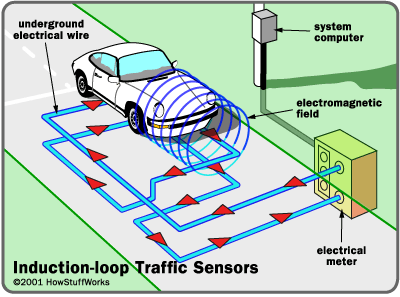
\includegraphics[width=8cm]{figures/induction-loop}
	\caption{Visualization of an induction loop}
	\label{induction-loop}
\end{figure}

In-pavement sensors are directly embedded into the street. Common examples for these are the well known inductive loop (see \autoref{induction-loop}), pneumatic road tubes and piezo-electric sensors. Inductive loops measure the inductance in their electric loop, piezo-electric sensors and pneumatic tubes measure the pressure applied on the road, to detect cars. Depending on the implementation, these sensors can not only detect a vehicle, but also classify vehicles based on weight or size. The speed of passing vehicles can usually not be detected directly, but by combining multiple of these simple sensors, is is possible to estimate the speed of the vehicles.
The main advantage of these sensors is the cost and the simple installation. The obvious downside of in-pavement sensors is the fact that damages in the pavement will lead to damages in the sensors.

Over-road sensors are mounted somewhere over the street. Usual mounting points are existing traffic signs and traffic lights. The technologies used for these sensors vary in a wide range: Infrared, radar, laser, optical cameras, sound and more. They differ in precision and use-cases. Most of them can measure not just the passage of vehicles, but also speed, vehicle class, license plates and more. These sensors do not suffer from the problems with in-pavement sensors, but have a new set of problems. Sensor that work optically are often affected by bad weather conditions that introduce to much noise in the picture. The main advantage of these sensors is the amount of additional information that can be collected and fast deployment.

\begin{figure}[ht]
	\centering
	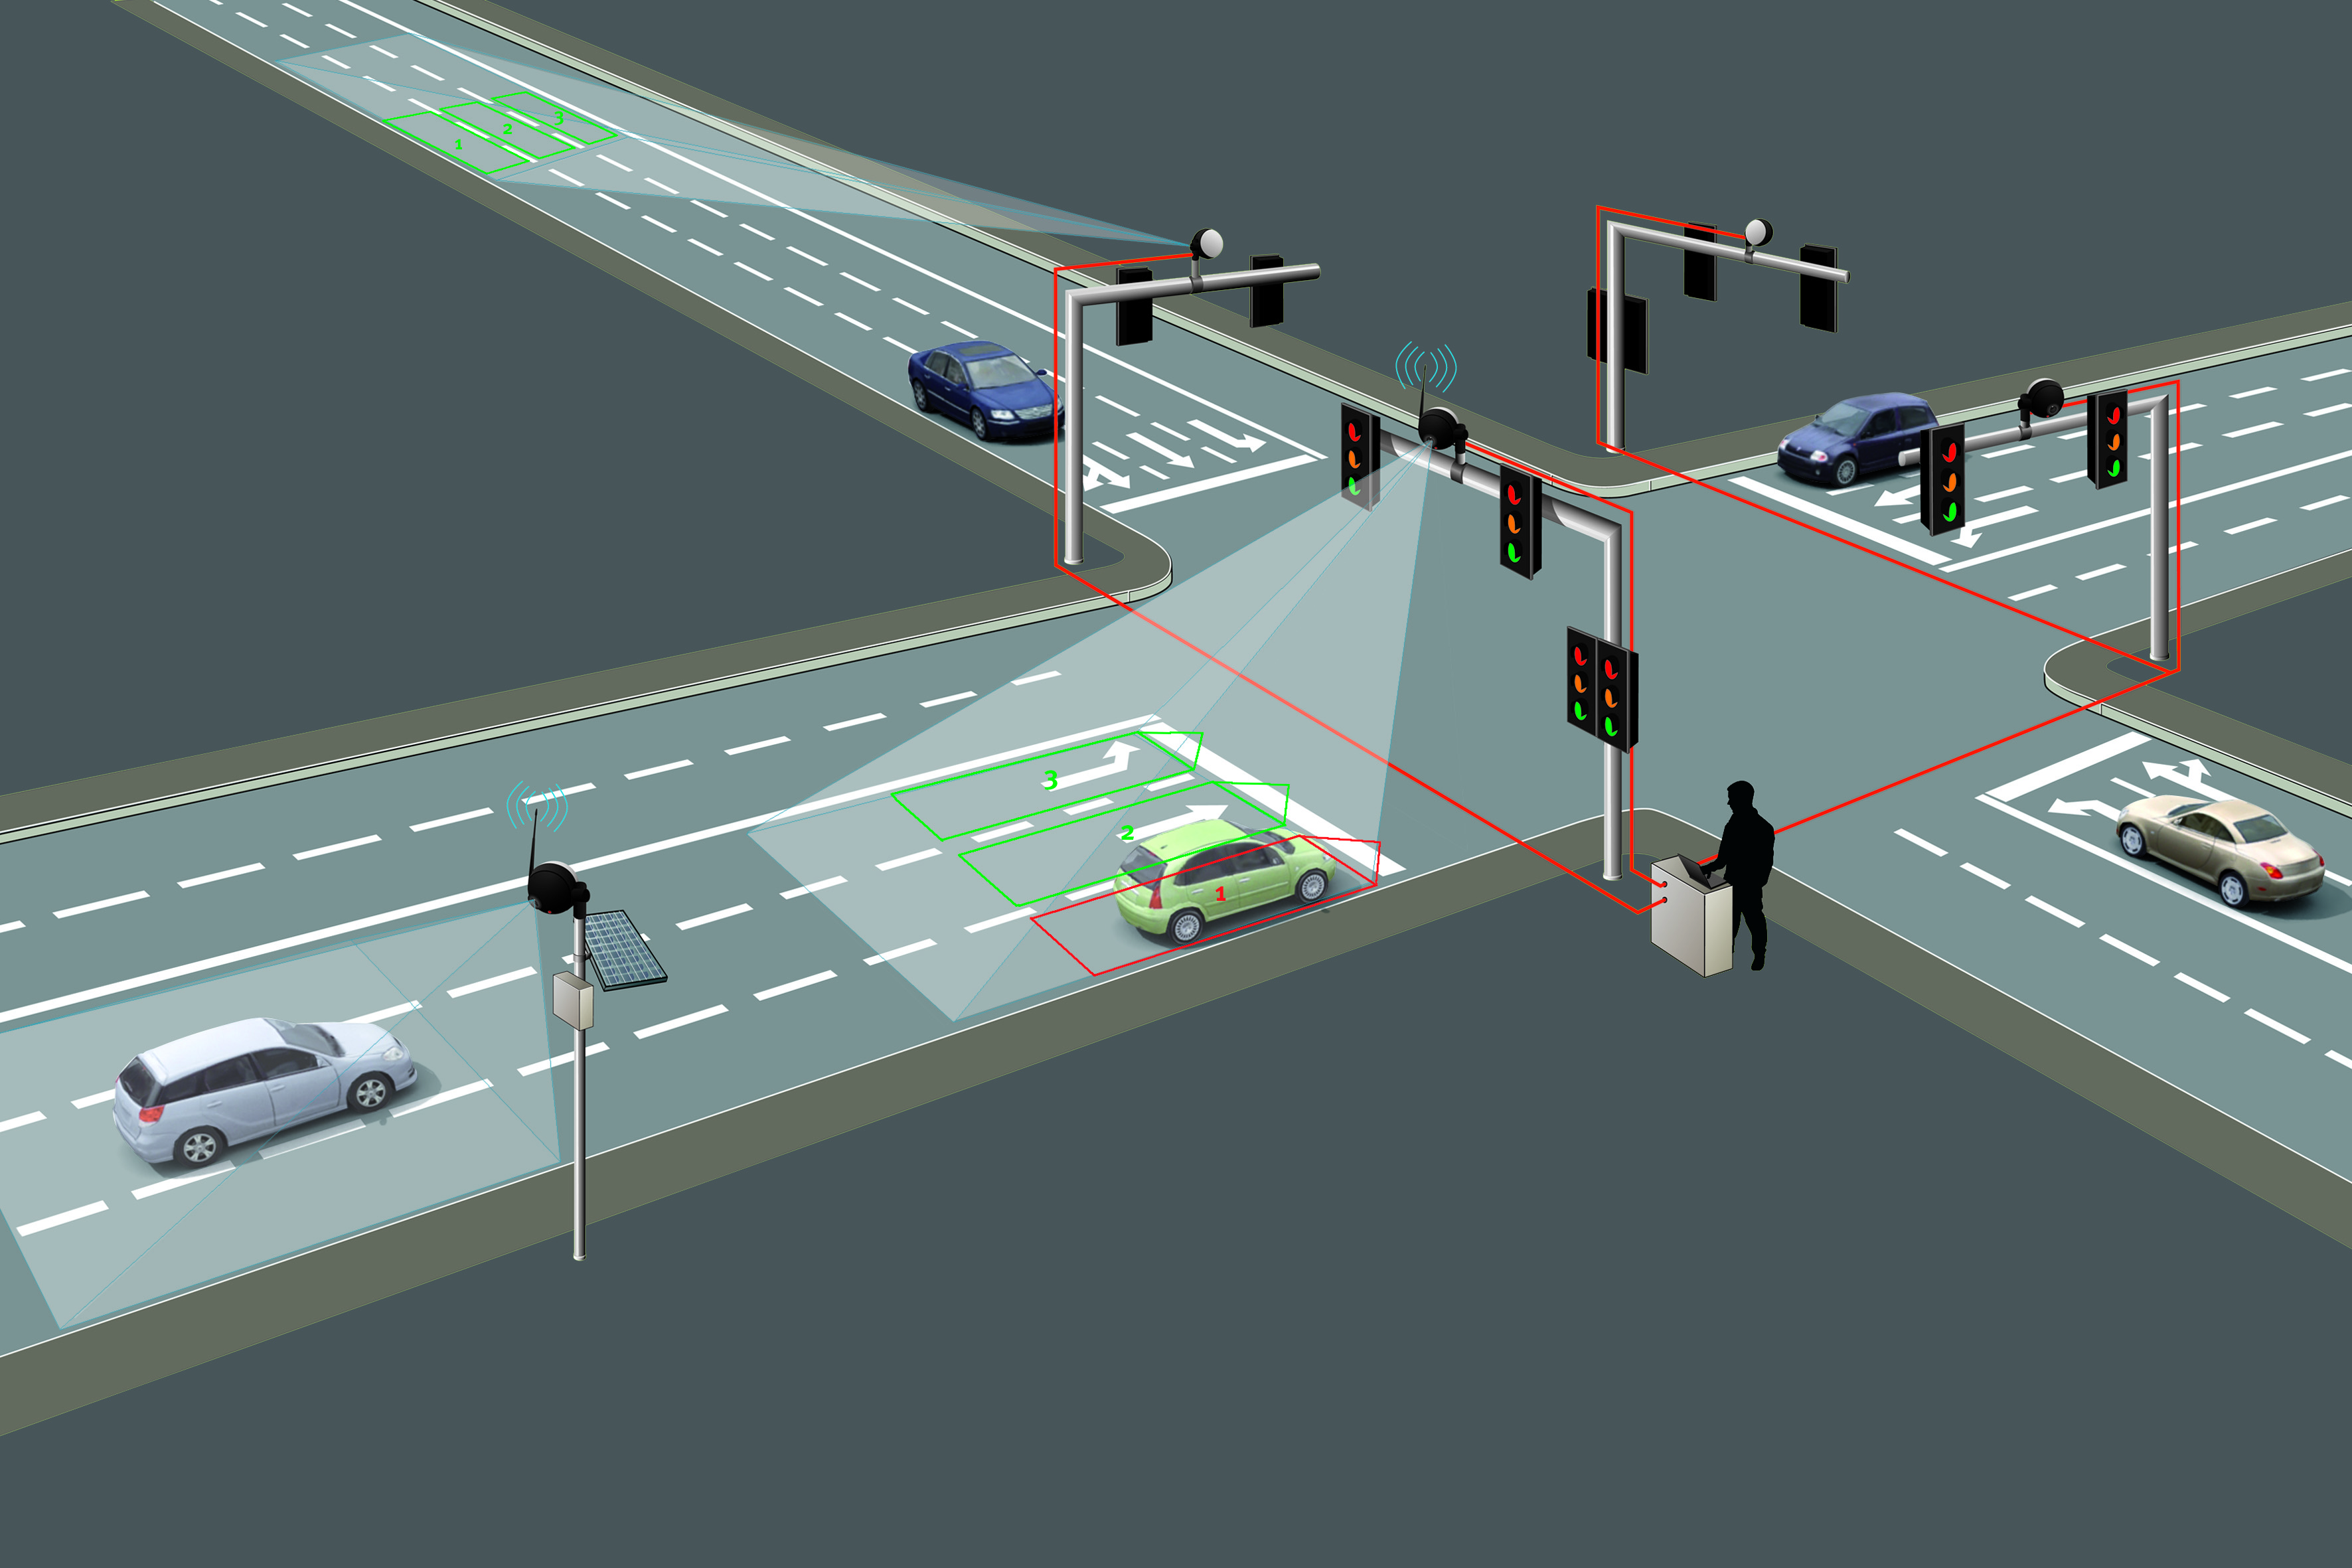
\includegraphics[width=8cm]{figures/overroad-sensor}
	\caption{Possible over-road sensor setup}
	\label{overroad-sensor}
\end{figure}

Given the sensors are in place and generate electrical signals for passing vehicles, these signals need to be collected somewhere. In simple systems, these sensors feed right back into local signal system. More advanced systems will collect the vehicle counts and other information in a central data center. Depending on the sensors the transmission is handled by the sensor itself or through additional devices. Modern sensors are directly connected to the Internet using the wireless broadband networks very common and reliable in cities. An example setup at an crossing can be seen in \autoref{overroad-sensor}.

\section{Artificial Neural Networks}

Artificial neural networks (ANNs) is an important field in machine learning and cognitive science. There are many different kinds of ANNs, but all have in common that they are inspired by biological neural networks, like the human brain. The big advantage of neural networks over algorithms that were explicitly developed for a task is that neural networks can learn behavior like classification from a set of example data and do not have to explicitly modeled. For this the neural network is modeled and the input and output vectors are defined. Then a set of example data i fed through the neural network and a learning algorithm tries to find a configuration of the neural network to get the desired outputs for the respective inputs. The ANNs form their own understanding of the problem while learning.

\begin{figure}[ht]
	\centering
  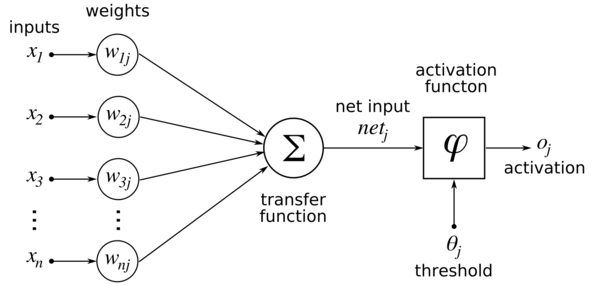
\includegraphics[scale=0.65]{figures/neuron_structure.png}
	\caption[Structure of a neuron]{Structure of a neuron \protect\footnotemark}
	\label{neuron}
\end{figure}
% https://upload.wikimedia.org/wikipedia/commons/thumb/6/60/ArtificialNeuronModel_english.png/600px-ArtificialNeuronModel_english.png
\footnotetext{wikipedia}

ANNs are typically a set of interconnected neurons. Figure \ref{neuron} shows the structure of a neuron. A neuron has a set of $n$ input variables $x_1, x_2, x_3, ..., x_n$ which either are connected to the output of another neuron or the input to the neural network that is given to the network by the user. Each input variable is multiplied with a weight $w_1j, w_2j, w_3j, ..., w_nj$ where $j$ is the iteration of the weight. All of the products of the variables and their specific weights are then summed and passed to an activation function that determines what the output of the neuron is.

\begin{figure}[ht]
	\centering
  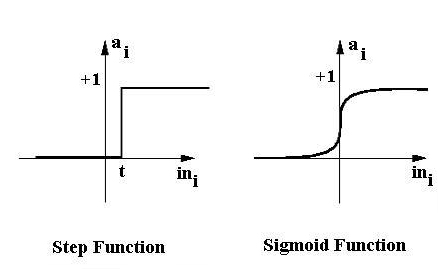
\includegraphics[scale=0.6]{figures/activation_functions.jpg}
	\caption[Step and sigmoid activation function]{Step and sigmoid activation function \protect\footnotemark}
	\label{activation_functions}
\end{figure}
% http://www.cs.nott.ac.uk/~pszgxk/courses/g5aiai/006neuralnetworks/images/actfn002.jpg
\footnotetext{interwebs}

Examples for the activation function would be a step function that just compares the value to a threshold and puts out 0 or 1 or a sigmoid function that puts out a value between 0 and 1. A plot of both can be seen in figure \ref{activation_functions}. $t$ in the case of the step function is a threshold that the input value has to pass to activate the neuron. But in most applications the step function is used because it can differentiate better. The output can then be given to the connected neurons or the output of the neural network.

An important aspect of ANNs is how the neurons are interconnected. The most basic structure of ANNs are feedforward neural networks. In this model the neural network is divided into layers and every layer only passes its information to the next layer. Thus, the input is fed forward through the layers until it is at the output layer. In contrast to that there are recurrent neural networks that allow the graph of neurons to have cycles. This allows the network to have some kind of memory and keep values to use in later iterations. An example for the use of recurrent neural networks would be a word processor that takes single words but can process whole sentences by memorizing what words were already passed through. There are a lot of sub categories of these structures and other architectures of ANNs, but feedforward and recurrent is the most important differentiation and the most relevant for this thesis.

\begin{figure}[ht]
	\centering
  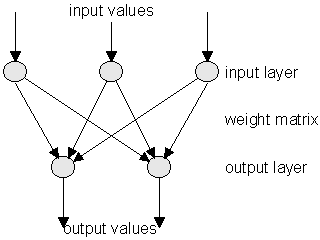
\includegraphics[scale=0.9]{figures/perceptron.png}
	\caption[Structure of a perceptron]{Structure of a perceptron \protect\footnotemark}
	\label{perceptron}
\end{figure}
% http://www.nnwj.de/uploads/pics/1_2-perceptron.gif
\footnotetext{interwebs}

Feedforward neural networks that only have an input layer and an output layer are called perceptrons. Such a network is shown in figure \ref{perceptron} They are the simplest kind of neural network, but they are very limited in their use. Because a neuron can only distinguish between two categories a neural network with only two layers is not even able to map a logical XOR. This is also known as the problem of linear separability. The advantage of this kind of neural network is that it does not need a lot of learning data and can use a really simple learning algorithm called the delta rule.

The delta rule is probably one of the most simple learning rules. It calculates a weight delta $\Delta w_{ji}$ for every $i$-th weight of neuron $j$ like this:

\begin{center}
	$\Delta w_{ji} = \alpha (t_j  y_j)g'(h_j)x_i$
\end{center}

With $\alpha$ being the learning, which directs how fast the network is reacting to trends, $t_j$ the target output, $y_j$ the actual output, $g$ being the activation function, $h_j$ the sum of the weighted inputs and $x_i$ the $i$-th input. This weight delta is then applied to the actual weight of the input. It is pretty easy to see how this works. The higher the difference between the target output of the neuron and the actual input, the higher the impact on the weight and the sign of this difference also defines in which direction the weight changes. The derivation of the activation function shows high values when the sum of the weighted inputs is near the threshold, thus the neuron is uncertain and a slight change in the weights could adjust the decision in one or the other direction. Furthermore the higher the input value the higher the change in the weight because it impacts the output more than lower input values.

\begin{figure}[ht]
	\centering
  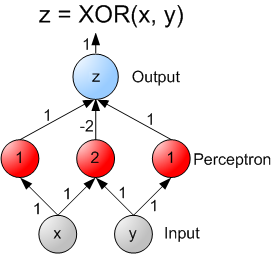
\includegraphics[scale=0.7]{figures/multilayer_XOR.png}
	\caption[Structure of a multilayer perceptron that implements an XOR]{Structure of a multilayer perceptron that implements an XOR \protect\footnotemark}
	\label{multilayer_XOR}
\end{figure}
% https://upload.wikimedia.org/wikipedia/commons/7/7b/XOR_perceptron_net.png
\footnotetext{wikipedia}

A bit more complex than perceptrons are multilayer perceptrons. They not only have an input and an ouput layer, but also one to several hidden layers that get fed from the previous layer and feed into the following layer. With this architecture more complex problems like XOR can be solved. The structure and weights of an XOR neural network are shown in figure \ref{multilayer_XOR}

Above was already shown how learning in simple ANNs takes place, but besides the function that determines how much a weight of a neuron changes, ANNs are also divided by the form of learning. This depends on how the learning set given to the neural network is created and composed. In the following the three most popular are described, being supervised learning, unsupervised learning and reinforcement learning. With supervised the learning set consists of pairs of input and output vectors and it thrives to adjust the weights of the neural network so that it maps the function described by the learning set. Then there is unsupervised learning which just takes for example a cost function, that calculates some costs from the input and output of the ANN, and a learning set, only consisting of data, and tries to minimize the cost function by adjusting the weights. The third possible scenario is reinforcement learning. This happens when there is no data set to learn from, but an agent interacts with some world and learns what interactions are good and what are bad by observing the effects. This is for example used when an artificial intelligence that plays chess is playing against itself to get better.

A problem with neural networks is that the higher the complexity of the network, its input and output vectors get, the higher is the demand for more learning data to get good results in the end. This is especially problematic for supervised learning algorithms because then the data has to be tagged by humans. This problem can be somewhat solved with reinforcement learning because it does not need the huge amounts of input from a human who is slow. This has to be taken into account when weighing between detail of the input and output and the amount of learning data needed.